%!TEX encoding = UTF-8 Unicode
%!TEX root = ../lect-w14.tex

%%%


%http://tex.stackexchange.com/questions/135393/how-to-draw-bar-pie-chart
\definecolor{c1}{RGB}{220,57,18}
\definecolor{c2}{RGB}{255,153,0}
\definecolor{c3}{RGB}{102,140,217}
\definecolor{c4}{RGB}{16,150,24}
\definecolor{c5}{RGB}{153,0,153}




\makeatletter

\tikzstyle{chart}=[
    legend label/.style={font={\scriptsize},anchor=west,align=left},
    legend box/.style={rectangle, draw, minimum size=5pt},
    axis/.style={black,semithick,->},
    axis label/.style={anchor=east,font={\tiny}},
]

\tikzstyle{bar chart}=[
    chart,
    bar width/.code={
        \pgfmathparse{##1/2}
        \global\let\bar@w\pgfmathresult
    },
    bar/.style={very thick, draw=white},
    bar label/.style={font={\bf\small},anchor=north},
    bar value/.style={font={\footnotesize}},
    bar width=.75,
]

\tikzstyle{pie chart}=[
    chart,
    slice/.style={line cap=round, line join=round, very thick,draw=white},
    pie title/.style={font={\bf}},
    slice type/.style 2 args={
        ##1/.style={fill=##2},
        values of ##1/.style={}
    }
]

\pgfdeclarelayer{background}
\pgfdeclarelayer{foreground}
\pgfsetlayers{background,main,foreground}


\newcommand{\pie}[3][]{
    \begin{scope}[#1]
    \pgfmathsetmacro{\curA}{90}
    \pgfmathsetmacro{\r}{1}
    \def\c{(0,0)}
    \node[pie title] at (90:1.3) {#2};
    \foreach \v/\s in{#3}{
        \pgfmathsetmacro{\deltaA}{\v/100*360}
        \pgfmathsetmacro{\nextA}{\curA + \deltaA}
        \pgfmathsetmacro{\midA}{(\curA+\nextA)/2}

        \path[slice,\s] \c
            -- +(\curA:\r)
            arc (\curA:\nextA:\r)
            -- cycle;
        \pgfmathsetmacro{\d}{max((\deltaA * -(.5/50) + 1) , .5)}

        \begin{pgfonlayer}{foreground}
        \path \c -- node[pos=\d,pie values,values of \s]{$\v\%$} +(\midA:\r);
        \end{pgfonlayer}

        \global\let\curA\nextA
    }
    \end{scope}
}

\newcommand{\legend}[2][]{
    \begin{scope}[#1]
    \path
        \foreach \n/\s in {#2}
            {
                  ++(0,-10pt) node[\s,legend box] {} +(5pt,0) node[legend label] {\n}
            }
    ;
    \end{scope}
}


\ifkompendium\else

\begin{Slide}{Sista veckan:}

  \begin{itemize}
    \item Uppsamling på \Emph{resurstider} för att uppnå tentakriteriet: \\ gör klart och redovisa \Alert{alla} labbar och projektet

    \item Erfarenhet visar att det är på \Emph{första} \Alert{ordinarie} tentan du har din bästa chans! 

    \item Om du får problem att uppnå tentakriteriet före jul så kontakta kursansvarig för en individuell bedömning av vägen framåt.
  \end{itemize}

\end{Slide}



\Subsection{Repetition forts.}

\begin{Slide}{På begäran!}
\url{http://cs.lth.se/pgk/wish}
% 2018 \url{https://goo.gl/forms/n4mxwjcAyAuF9Y8k2}
% 2019 \url{https://forms.gle/z3FvAXnviiqMjbieA}
\end{Slide}

% \begin{Slide}{Föränderlig punkt  i Scala och Java}\SlideFontSmall
% I Scala:
% \begin{Code}
% class Point(var x: Int, var y: Int)
% \end{Code}
% \pause
% I Java:
% \begin{Code}[language=Java,basicstyle=\ttfamily\SlideFontSize{5.2}{6}]
% public class JPoint {
%     private int x;
%     private int y;

%     public JPoint(int x, int y){
%         this.x = x;
%         this.y = y;
%     }

%     public int getX(){
%         return x;
%     }

%     public int getY(){
%         return y;
%     }

%     public void setX(int x){
%         this.x = x;
%     }

%     public void setY(int y){
%         this.y = y;
%     }
% }
% \end{Code}
% \end{Slide}

% \begin{Slide}{Punkt med räknare och setter i Scala}
% Övning: lägg till getter och setter för y-koordinaten.
% \begin{Code}
% class Point(private var myX: Int, private var myY: Int){
%   import Point._
%   def x = myX
%   def x_=(value: Int): Unit = {
%     myX = value
%   }
%   myCount += 1   // kod i klasskroppen körs vid konstruktion
% }

% object Point {
%   private var myCount = 0
%   def count = myCount
% }
% \end{Code}
% \SlideFontSmall
% Man brukar kalla privata attribut som har getter (och ev. setter) för något i stil med \code{myX} eller vanligare \code{_x} för att namnet inte ska krocka med getter/setter.
% \end{Slide}



% \begin{Slide}{Punkt med räknare i Java}

% \begin{Code}[language=Java,basicstyle=\ttfamily\SlideFontSize{5.2}{6}]
% public class JPoint {
%     private int x;
%     private int y;

%     static private int count = 0;  // static: finns bara en upplaga av detta attribut

%     public JPoint(int x, int y){
%         this.x = x;
%         this.y = y;
%         count++;
%     }

%     public int getX(){
%         return x;
%     }

%     public int getY(){
%         return y;
%     }

%     public void setX(int x){
%         this.x = x;
%     }

%     public void setY(int y){
%         this.y = y;
%     }

%     static public int getCount(){
%        return count;
%     }
% }
% \end{Code}


% \end{Slide}

% \begin{Slide}{Gamla Java-kursen}
% Du hittar genomgång av olika Java-begrepp i gamla Java-kursen som finns här: \\\vspace{1em}
% \url{http://cs.lth.se/eda016/}
% \\\vspace{2em}

% Övning: träna på att översätta Java-exempel till scala

% \end{Slide}


\Subsection{Utblick}

% \begin{Slide}{Framtidens (data)ingenjör}
% Vårt utbildninguppdrag vid institutionen för Datavetenskap:
% \begin{itemize}
%   \item Utbilda \Emph{dataingenjörer} för \Alert{framtidens} arbetsmarknad
%   \item Säkerställa att alla typer av LTH-ingenjörer har \Emph{tillräckliga} kunskaper i datavetenskap och modern systemutveckling
%   \item Förbereda för \Emph{livslångt lärande} inom \Alert{datavetenskap}: rätt grundkunskaper för att kunna lära sig ny teknik/forskning
%   \item Tillgodo se behovet av den \Emph{djupa datavetenskapliga kompetens} som dagens och morgondagens näringsliv är i så \Alert{skriande behov} av: \\
%   \url{https://computersweden.idg.se/2.2683/1.693037/bransch-it-jobb} \\
% \end{itemize}
% \Alert{''Nytt branschlarm: Behövs 70000 fler som jobbar med it''}
% \end{Slide}
%
% \begin{Slide}{Vad är de två allra största utmaningarna för framtiden inom software engineering?}
%   \begin{enumerate}
%     \item Kompetensbristen
%     \item
%     \pause Att hantera den ständigt ökande \Alert{komplexiteten}
%   \end{enumerate}
%   \pause(Del)lösning: \pause \Emph{kraftfullare abstraktionsmekanismer}
% \end{Slide}
%
%
% \begin{Slide}{Kraftfulla abstraktionsmekanismer i Scala}\SlideFontTiny
% \setlength{\leftmargini}{-1em}
% \begin{itemize}
% \item Funktioner som parametrar:
% \begin{Code}
% def sort[T](xs: Vector[T], lessThan: T => Boolean): Vector[T] = ???
% \end{Code}
%
% \item Extension methods (metodutvidgning):
% \begin{Code}
% implicit class DecoratePerson(p: Person) {
%   def lessThan(other: Person): Boolean = ???
% }
% \end{Code}
%
% \item Implicita parametrar:
% \begin{Code}
% def sort[T](xs: Vector[T])(implicit ord: Ordering[T]): Vector[T] = ???
% \end{Code}
%
% \item Implicita konverteringar mellan typer
%
% \item Typklasser (jmf Haskell) i Scala med traits + implicita värden
%
% \item Scala 3.0: Implicita funktioner för att abstrahera över kontext
%
% \end{itemize}
% {\noindent\tiny Föredrag av Odersky: \\
% ''Plain functional programming'' \url{https://youtu.be/YXDm3WHZT5g}\\
% ''What to leave implicit?'' \url{https://youtu.be/Oij5V7LQJsA?list=PLLMLOC3WM2r5Ei2mnSHCD-ZD04AXovttL}}
% \end{Slide}
%
%
% \begin{Slide}{Framtidens kurser för D-are}
% \begin{itemize}
%   \item \href{http://cs.lth.se/utbildning/}{Undervisningen i Datavetenskap} har fördubblats på 5 år
%   \item D-programmet utvecklas: flera nya kurser införda/på gång
%   \item Exempel på kurser som direkt bygger på grundkursen i programmering med Scala, \code{pgk}:
% \begin{itemize}
% \item Fördjupningskursen (Java)
% \item \Alert{Ny sedan 2016:} Utvärdering av programvarusystem (R)
% \item \Alert{Ny sedan 2016:} Diskreta strukturer (Clojure)
% \item Programvaruutveckling i grupp (Java)
% \item Objekt-orienterad modellering och design (Java)
% \item \Alert{Numera obligatorisk:} Funktionsprogrammering (Haskell)
% \end{itemize}
% \item Exempel på pågående/föreslagen kursutveckling:
% \begin{itemize}
%   \item Machine Learning
%   \item Concurrency, distribution, real-time embedded systems
%   \item Open Source Software Engineering
%   \item Development for web apps, cloud, back-end, (front-end)
%   \item Tool chain for continuous software engineering
% \end{itemize}
% \end{itemize}
% \end{Slide}
%
%
% \begin{Slide}{Mål med nya grundkursen i Scala}
% \begin{itemize}
%   \item Hantera stora spridningen i förkunskaper. Andel nybörjare:
%   \begin{itemize}
%     \item 2015: ca 20\% har aldrig kodat före kursstart
%     \item 2016: ca 30\% har aldrig kodat före kursstart
%     \item 2017: ca 40\% har aldrig kodat före kursstart
%   \end{itemize}
%   \item Hantera stora spridningen i förmåga att ta sig över trösklar:
%   \begin{itemize}
%     \item Många studenter har hög ambition och hög motivation
%     \item Några studenter har stora svårigheter i början
%   \end{itemize}
%   \item Modernisera innehåll och pedagogik:
%   \begin{itemize}
%     \item grundläggande objektfunktionell programmering
%     \item använda ett modernt, kraftfullt samlingsbibliotek
%     \item oföränderliga datastrukturer
%     \item samarbete mellan studenter
%     \item allt kursmaterial är fri öppenkällkod med studentdeltagande i den kontinuerliga utvecklingen:
%     \url{https://github.com/lunduniversity/introprog}
%   \end{itemize}
% \end{itemize}
% \end{Slide}
%
%
% \begin{Slide}{Innehåll i nya grundkursen i Scala}\SlideFontTiny
% Kursens hemsida: \textbf{\url{http://cs.lth.se/pgk}} \\ \vspace{1em}
%
% \noindent\resizebox{0.8\columnwidth}{!}{\fontsize{8}{10}\selectfont
% %!TEX encoding = UTF-8 Unicode
\begin{tabular}{l|l|l|l}
\textit{W} & \textit{Modul} & \textit{Övn} & \textit{Lab} \\ \hline \hline
W01 & Introduktion            & expressions & kojo            \\
W02 & Kodstrukturer           & programs    & --              \\
W03 & Funktioner, Objekt      & functions   & bugs            \\
W04 & Datastrukturer          & data        & pirates         \\
W05 & Sekvensalgoritmer       & sequences   & cards           \\
W06 & Klasser, Likhet         & classes     & turtlegraphics  \\
W07 & Arv, Gränssnitt         & traits      & turtlerace-team \\
KS  & KONTROLLSKRIVN.         & --          & --              \\
W08 & Mönster, Undantag       & matching    & chords-team     \\
W09 & Matriser, Typparametrar & matrices    & maze            \\
W10 & Sökning, Sortering      & sorting     & surveydata-team \\
W11 & Scala och Java          & scalajava   & lthopoly-team   \\
W12 & Trådar                  & threads     & life            \\
W13 & Design                  & Uppsamling  & Projekt         \\
W14 & Tentaträning            & Extenta     & --              \\
T   & TENTAMEN                & --          & --              \\
\end{tabular}

% }
%
% \vspace{1em}
% Kursmaterial är öppen källkod: \textbf{\url{https://github.com/lunduniversity/introprog}}
% \end{Slide}
%
%
%
% \begin{Slide}{Förstaspråk på LTH}%\small
% Historiska förstaspråk på LTH för D-are:
% \begin{table}
% \begin{tabular}{l l}
% (Algol) & (förhistoria\footnote{Scalas uppfinnare Prof. Martin Odersky vid EPFL i Schweiz har skapat stora delar av Java-kompilatorn. Han var doktorand hos Prof. Niklaus Wirth, som ligger bakom Algol, Pascal, Modula etc.}, programmering med hålkort) \\
%  Pascal & 1982, CSE program started\\
%  Simula &  1990\\ % , first OO language; Invented in Scandianiva
%   Java &  1997 \\
% \Emph{Scala} &  2016 \\
% \end{tabular}
% \end{table}
%
% \end{Slide}

%
% \begin{Slide}{Varför Scala? -- ur pedagogisk synvinkel}
% \Emph{Lätt} för nybörjare och \Alert{intressant} för icke-nybörjare:
% \begin{itemize}
% \item Enhetlig semantik; alla värden är objekt
% \item Koncis syntax: drunknar inte i ''bokstavssoppa''
% \item Uttrycksfull semantik: kan demonstrera många koncept
% \item Statisk typning hjälper till med förståelse av abstraktioner
% \item Statisk typning gör att kompilatorn kan hitta buggar tidigt
% \item Interaktivt lärande med Scala REPL
% \item Multi-paradigm, pragmatiskt: \\ imperativt, objekt-orienterat, funktionellt
% \item Modernt språk som utvecklas med forskning och praxis
% \item Språket och verktygen är fri öppen källkod
% \end{itemize}
% \pause {\SlideFontSmall Några \Alert{risker} men som vi identifierade men som \Emph{inte} visat sig vara problem: verktygsmognad, tillgång till kursmaterial för nybörjare, kritisk massa i communityn, industriell acceptans och relevans.}
% %\begin{itemize}\fontsize{9}{10}\selectfont
% %\item Tools not becoming mature fast enough?
% %\item Lack of beginner-oriented teaching material?
% %\item Future industrial relevance?
% %\item Critical mass of community?
% %\end{itemize}
% \end{Slide}
%
% \begin{Slide}{Varför inte Python? -- ur pedagogisk synvinkel}\SlideFontSmall
% Det finns många fördelar med Python som även gäller Scala, t.ex. enhetligt och kraftfullt standardbibliotek och koncis syntax, men också många nackdelar som inte Scala har:
% \begin{itemize}
% \item \Alert{Indenteringssyntaxen} kan göra det svårare att förstå koncepten block, lokala variabler och namnrymd, speciellt precis i början av lärandet, och speciellt vid nästlade strukturer.
% \item \Alert{Avsaknad av typinformation} vid abstraktion och buggrättning - utan t.ex. parametertyper kan nybörjaren råka blanda ihop t.ex. om argument är samlingar eller enskilt element. Dynamisk typning ger onödiga svårigheter där kompilatorn annars kunde ha hjälpt till.
% \item Att (felstavade) variabler kan införas \Alert{utan deklaration} medför mycket svårhittade namnöverskuggningsbuggar även för icke-nybörjare.
% \item Att objektmodellen är så pass långt från "riktig" objektorientering gör att de möjliga \Alert{lärandemålen kring objektorientering begränsas} starkt.
%   \end{itemize}
% \end{Slide}


% \begin{Slide}{Betyg, D-are: 2015 Java; 2016 Scala}
%
%   2015 Java, januaritenta D, 91st
%
%   \pgfplotstableread{
%   betyg antal
%   0 12
%   3 04
%   4 26
%   5 49
%   }{\mydataFifteen}
%
%   \begin{minipage}{0.4\textwidth}
%   \hspace*{-0.0cm}
%   \begin{tikzpicture}[scale=0.8, every node/.style={scale=0.8}]
%       \begin{axis}[
%               ybar,
%               bar width=.5cm,
%               width=\textwidth,
%               height=0.9\textwidth,
%               symbolic x coords={0,3,4,5},
%               xtick=data,
%               nodes near coords,
%               nodes near coords align={vertical},
%               ymin=0,ymax=50,
%               ylabel={Antal},
%               xlabel={Betyg},
%           ]
%           \addplot table[x=betyg,y=antal]{\mydataFifteen};
%       \end{axis}
%   \end{tikzpicture}
%   \end{minipage}%
%   \begin{minipage}{0.3\textwidth}
%   \vspace*{-1cm}\hspace*{1.5cm}
%   \begin{tikzpicture}
%   [
%       pie chart,
%       slice type={NOLL}{c1},
%       slice type={TRE}{c4},
%       slice type={FYRA}{c2},
%       slice type={FEM}{c3},
%       pie values/.style={font={\small}},
%       scale=1.3, every node/.style={scale=0.8}
%   ]
%       \pie{}{13/NOLL,4/TRE,29/FYRA,54/FEM}
%       \legend[shift={(1.5cm,1cm)}]{{0}/NOLL,{3}/TRE, {4}/FYRA, {5}/FEM}
%   \end{tikzpicture}
%   \end{minipage}%
%
%
% \vspace*{1em}
%
% 2016 Scala, januaritenta D, 86st
% \pgfplotstableread{
% betyg antal
% 0 17
% 3 12
% 4 29
% 5 28
% }{\mydataSixteen}
%
% \begin{minipage}{0.4\textwidth}
% \hspace*{-0.0cm}
% \begin{tikzpicture}[scale=0.8, every node/.style={scale=0.8}]
%     \begin{axis}[
%             ybar,
%             bar width=.5cm,
%             width=\textwidth,
%             height=0.9\textwidth,
%             symbolic x coords={0,3,4,5},
%             xtick=data,
%             nodes near coords,
%             nodes near coords align={vertical},
%             ymin=0,ymax=50,
%             ylabel={Antal},
%             xlabel={Betyg},
%         ]
%         \addplot table[x=betyg,y=antal]{\mydataSixteen};
%     \end{axis}
% \end{tikzpicture}
% \end{minipage}%
% \begin{minipage}{0.3\textwidth}
% \vspace*{-1cm}\hspace*{1.5cm}
% \begin{tikzpicture}
% [
%     pie chart,
%     slice type={NOLL}{c1},
%     slice type={TRE}{c4},
%     slice type={FYRA}{c2},
%     slice type={FEM}{c3},
%     pie values/.style={font={\small}},
%     scale=1.3, every node/.style={scale=0.8}
% ]
%     \pie{}{20/NOLL,14/TRE,34/FYRA,33/FEM}
%     \legend[shift={(1.5cm,1cm)}]{{0}/NOLL,{3}/TRE, {4}/FYRA, {5}/FEM}
% \end{tikzpicture}
% \end{minipage}%
%
%
% \end{Slide}
%
%
%
%
% \begin{Slide}{Betygens värde i fördjupningskursen 2015:\\EDA016 Java => EDAA01 Java}
% \href{https://jsfiddle.net/dyb0kpvh/}{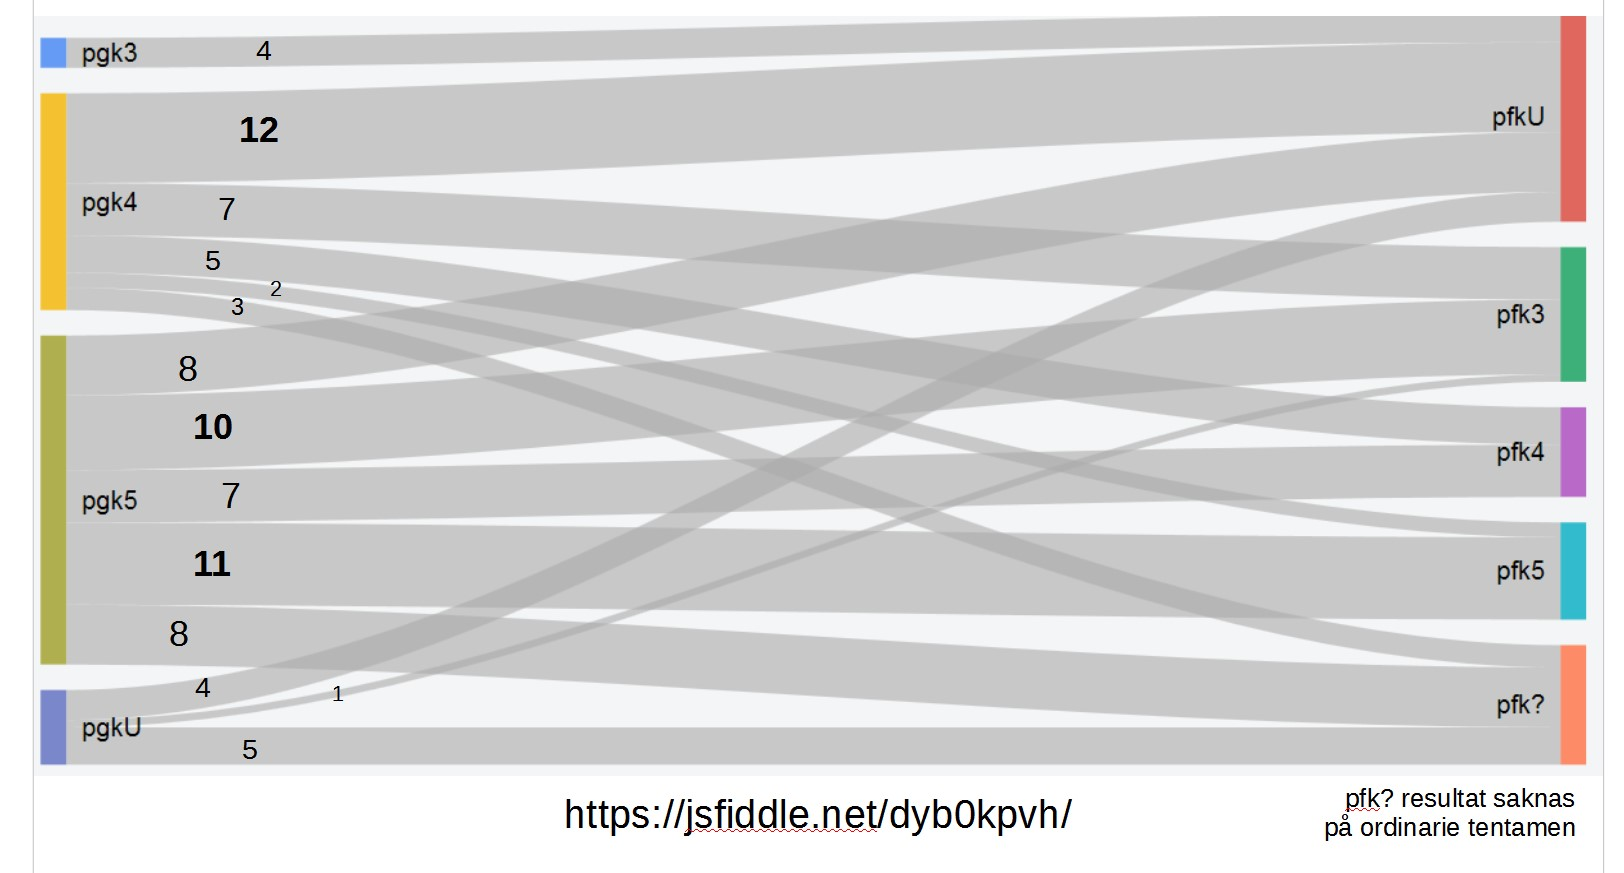
\includegraphics[width=1.05\textwidth]{../about/course-experience-first-year/img/2015}}
% \end{Slide}
%
% \begin{Slide}{Betygens värde i fördjupningskursen 2016:\\EDAA45 Scala => EDAA01 Java}
% \href{https://jsfiddle.net/wa7fr8po/}{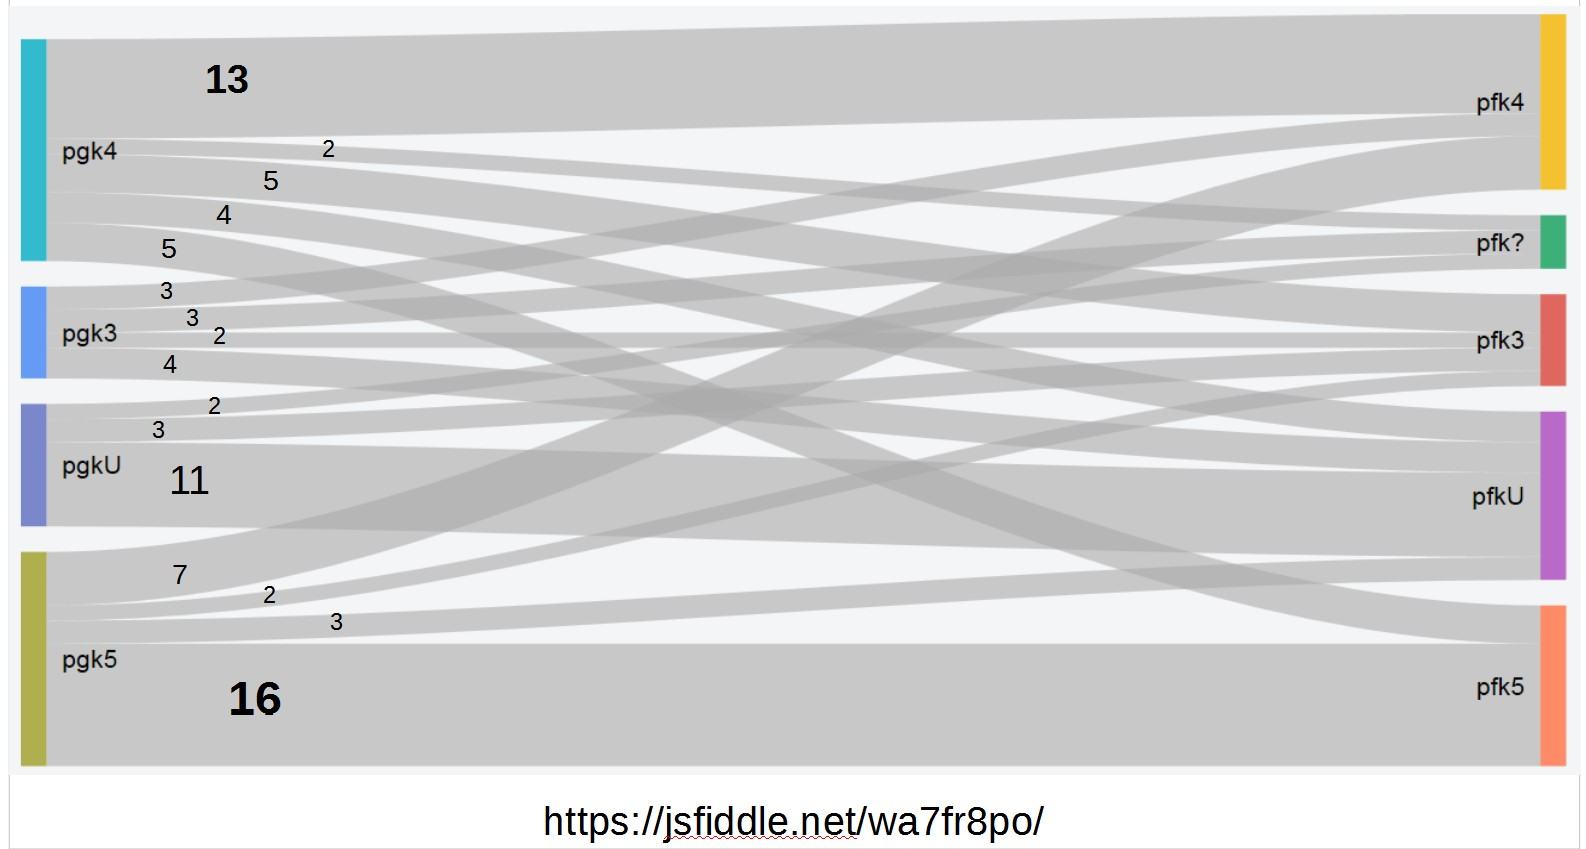
\includegraphics[width=1.05\textwidth]{../about/course-experience-first-year/img/2016}}
% \end{Slide}
%


% \begin{Slide}{Hur populärt blir Scala bland utvecklare i framtiden?}
% Mest älskade språk på \code{stackoverflow} (2016)
% 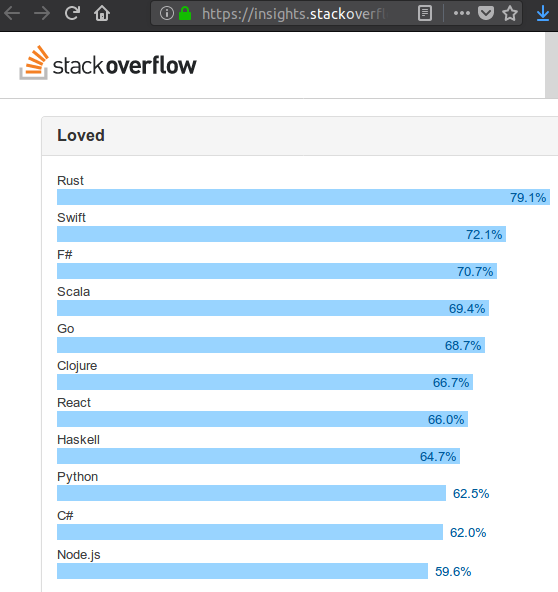
\includegraphics[width=0.9\textwidth]{../img/w14/most-loved-2016.png}
% \end{Slide}
%
% \begin{Slide}{Hur ser framtidens jobbmarknad för Scala ut?}\SlideFontTiny
%
% \hspace{-2.5em}\begin{minipage}{1.0\textwidth}
% Jobbmarknaden för Scala växer globalt och i Sverige:
%
% \begin{minipage}{0.48\textwidth}
% \href{www.indeed.com/jobtrends/q-scala.html}{www.indeed.com/jobtrends/q-scala.html}\\
% \vspace{1em}
% 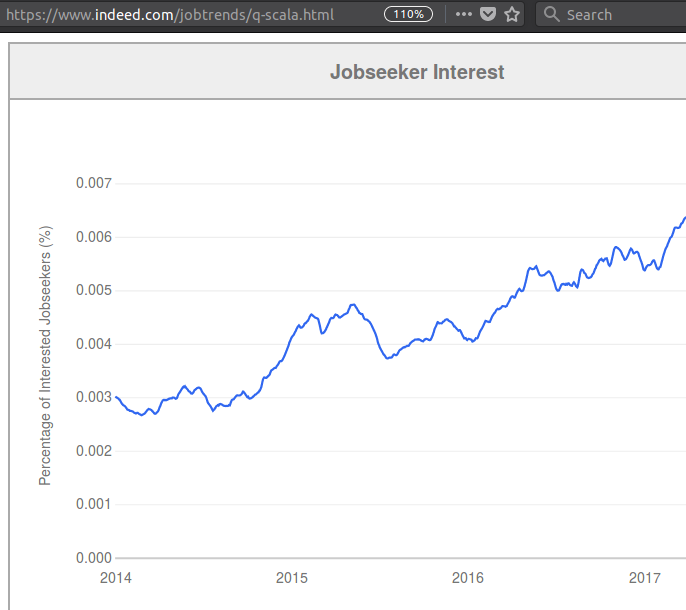
\includegraphics[width=1.0\textwidth]{../img/w14/scala-jobs-indeed-2017.png}~~
% \end{minipage}
% \hfill\begin{minipage}{0.48\textwidth}
% \vspace{1.25em}
% \href{https://www.linkedin.com/jobs/search/?keywords=scala&location=Sweden&locationId=se%3A0}{https://www.linkedin.com/jobs/search/?keywords=scala}\\
% 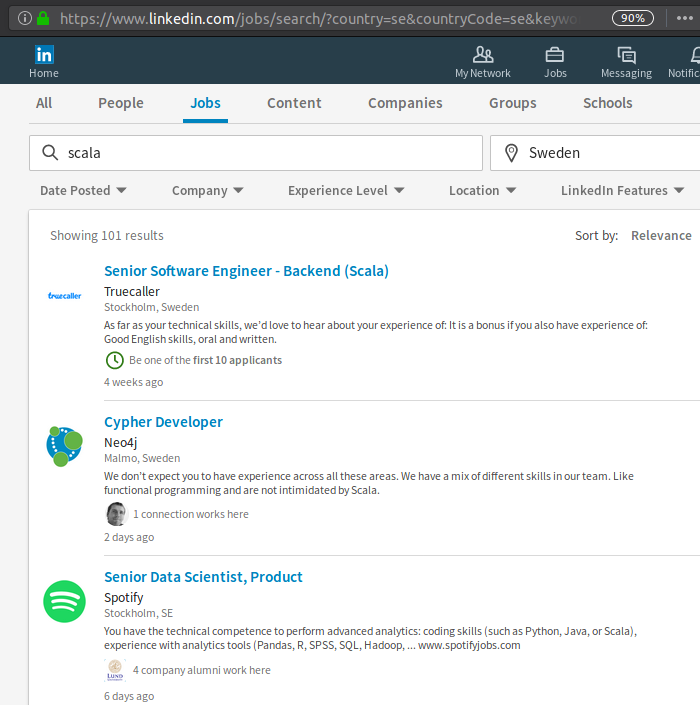
\includegraphics[width=1.2\textwidth]{../img/w14/scala-jobs-sweden-linkedin-2017-dec07.png}
% \end{minipage}
% \end{minipage}
% \end{Slide}



\begin{Slide}{Scala versus Python}
  \begin{itemize}
    \item 
    Två språk som blir allt mer populära för ''big data'' och AI: \\ Scala \& Python
    \item Intressant blogginlägg om vilket språk som funkar bäst som förstaspråk för de som ska bli systemutvecklare:
    {\tiny\url{https://medium.com/@drmarkclewis/picking-a-languages-for-introductory-cs-the-argument-againstpython-4331cca26cfa}}
    \item Hur ser framtiden ut för Scala?
  \end{itemize}
\end{Slide}


\begin{Slide}{Scala då, nu och i framtiden}\SlideFontSmall

{\SlideFontSize{7}{10}\url{
https://en.wikipedia.org/wiki/Scala_(programming_language)#Versions
}}

\begin{itemize}
\item Scala 1.0 (2003) första pre-release
\item Scala 2.0-2.9 (2006-2011) pionjärer: Twitter, LinkedIn, The Guardian, ...
\item Scala 2.10 (2013) brett genombrott, viktiga språkutvidgningar
\item Scala 2.11 (2014) allmän industriell spridning, stabilitet, prestanda, \\
{\SlideFontSize{7}{10}\url{
https://en.wikipedia.org/wiki/Scala_(programming_language)#Companies
}}
\item Scala 2.12 (2016) fokus på prestanda, snabbare bytekod med lambda i JVM Java 8
\item Scala 2.13 (2019) fokus på standardbiblioteket och \code{scala.collection}, migreringsverktyg för Scala 3
\item Scala 3.0~~(2021): \Alert{stort} \Emph{tekniksprång}:\\enum, top-level defs, @main, trait params, given, export, creator applications, ...,\\ "uppstädning" + förenklingar baserat på lärdomar från Scala 2.
\end{itemize}
\end{Slide}

\begin{Slide}{Scala 3 och Dotty}\SlideFontSmall
\begin{itemize}
\item Experimentkompilator och testmiljö inför Scala 3: \Emph{dotty} \url{http://dotty.epfl.ch/}
\begin{itemize}\SlideFontTiny
  \item Formell bas för Scala: DOT (en algebra för dependent object types)
  \item Städa upp språket (skippa vissa saker, t.ex. xml-litteraler)
  \item Prova nya språkkonstruktioner, t.ex. enum, top-level defs, @main, trait params, given, export, creator applications, ...,
  \item Nytt format för kodträd som kompletterar bytekod: \Emph{Tasty}\\
\end{itemize}
\item Flera ''backends'' som breddar Scalas användningsområde:
\begin{itemize}\SlideFontTiny
  \item \href{http://www.scala-js.org/}{scala-js.org}: dela kod+kompetens mellan backend och frontend
  \item \href{http://scala-native.org}{scala-native.org}: kör Scala kompilerat direkt ''på metallen''
  \item \href{http://scala-android.org}{scala-android.org}: skapa appar för mobilen
\end{itemize}
\item Några viktiga Scala-ramverk för stordata, massiv parallellism, AI:
\begin{itemize}\SlideFontTiny
  \item \href{https://akka.io/}{Akka} ramverk för skalbara parallella arkitekturer
  \item \href{https://spark.apache.org/}{Apache Spark} för parallell behandling av stordata i molnet, för AI, ML ...
  \item \href{https://www.playframework.com/}{Play framework} för moderna, skalbara webbappar
\end{itemize}
\end{itemize}
\end{Slide}


% \begin{Slide}{Roadmap för Scala 3.0}
%   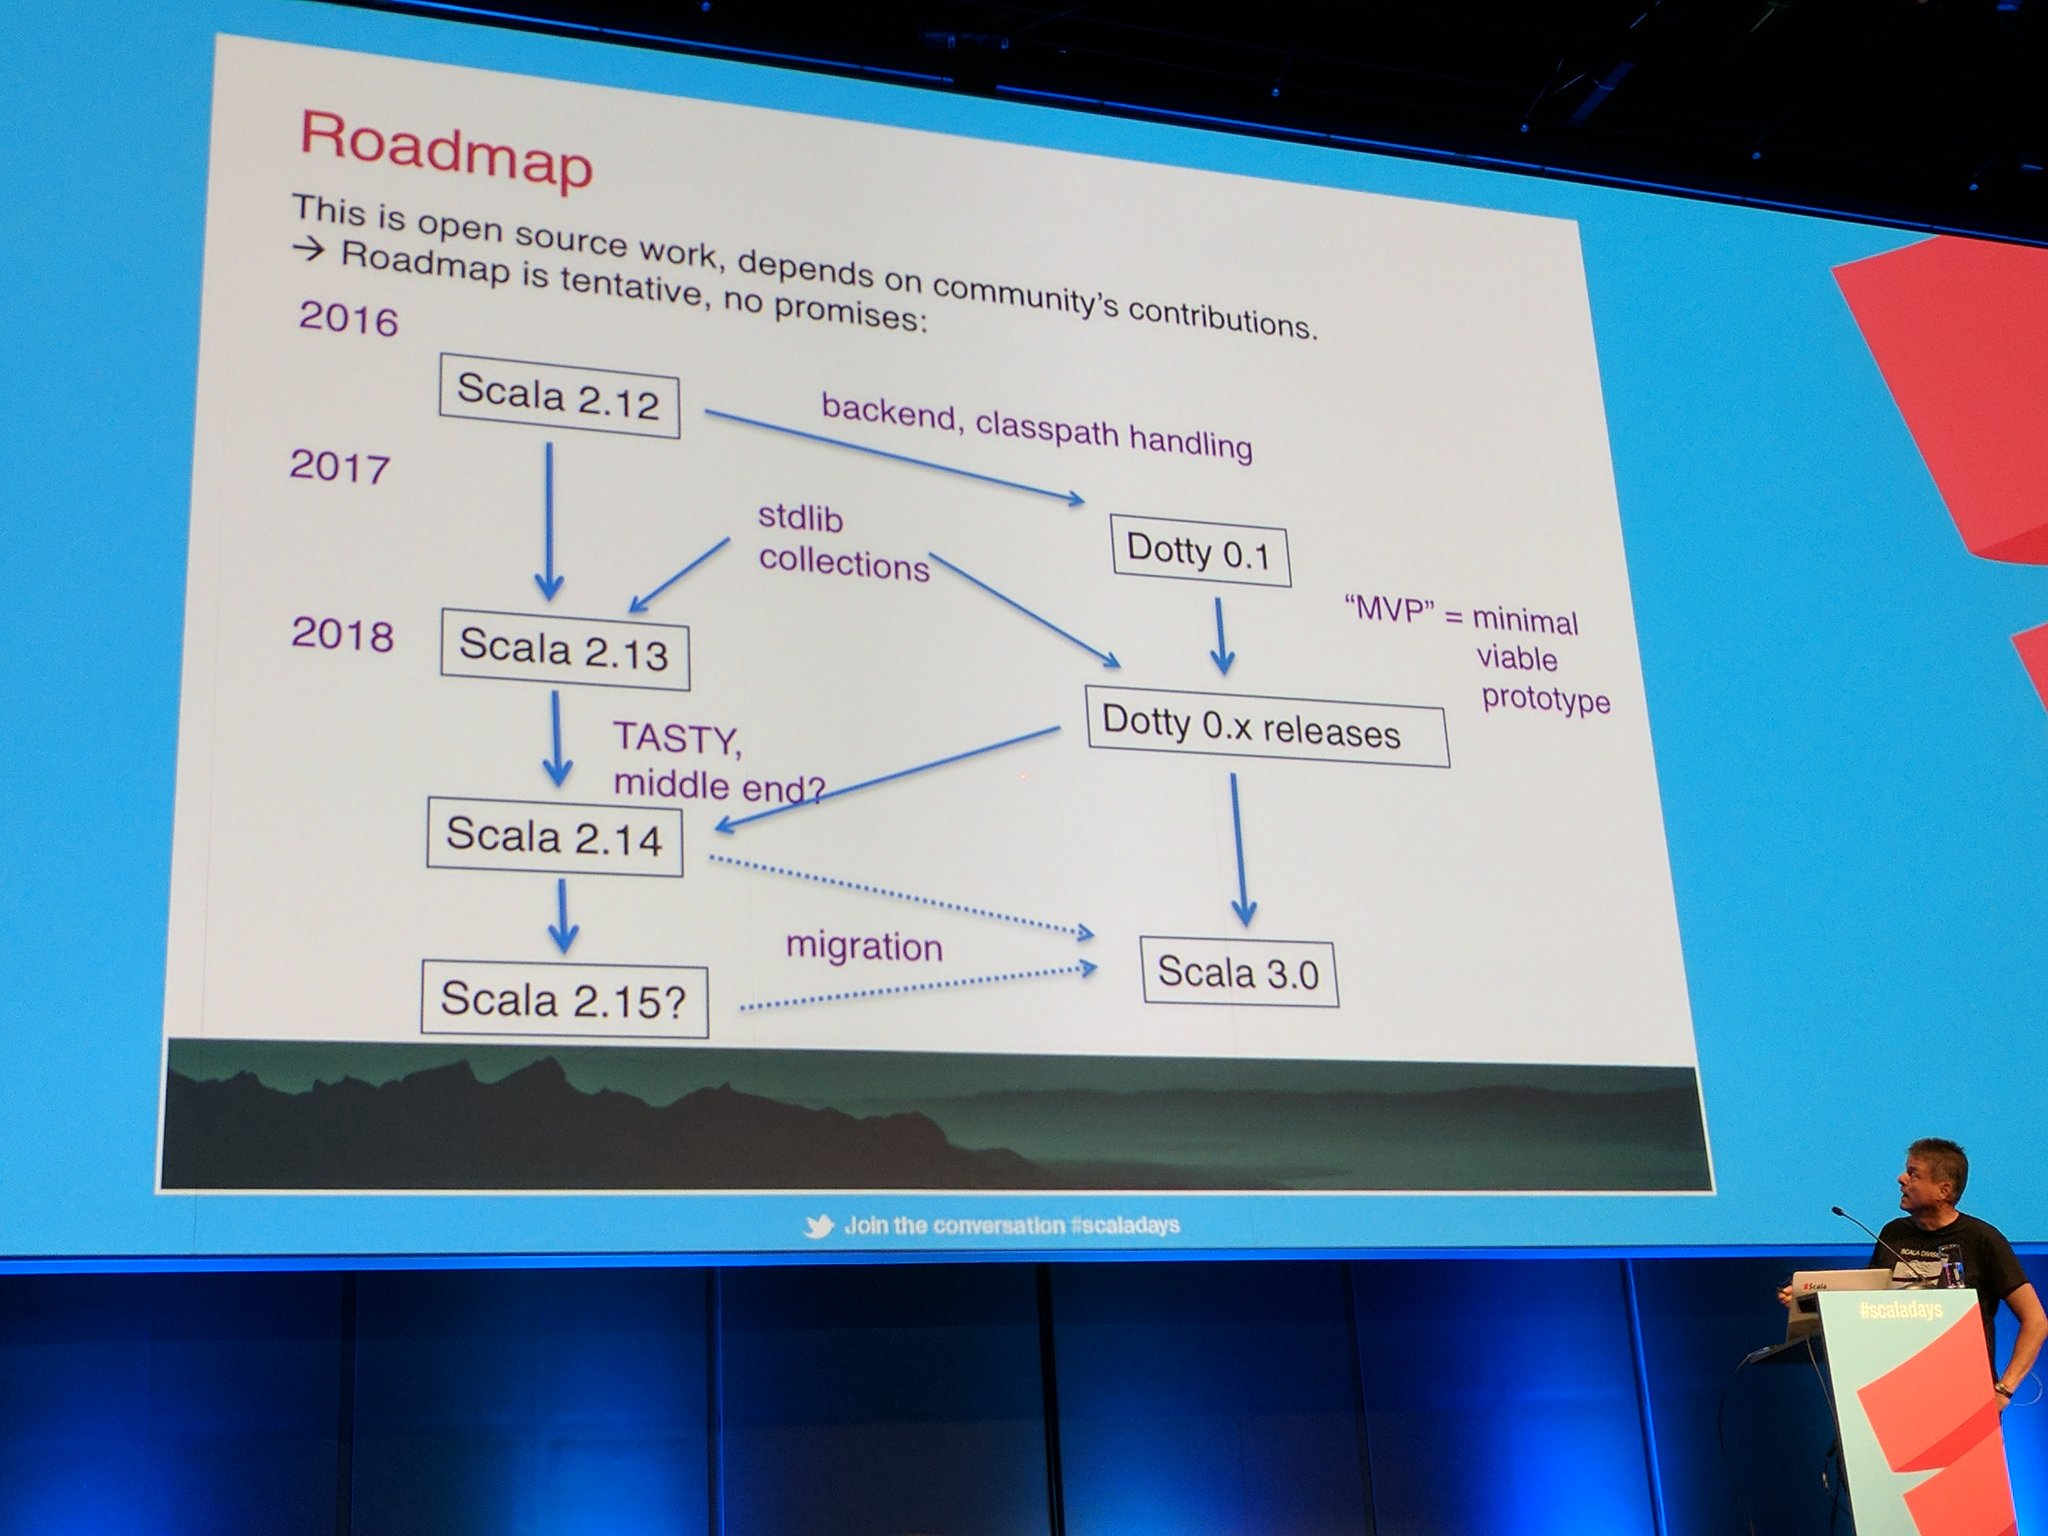
\includegraphics[width=0.9\textwidth]{../img/w14/scala-dotty-roadmap-odersky.jpeg}
% \end{Slide}



\begin{Slide}{Hur håller jag mig uppdaterad om Scalas utveckling?}
\begin{itemize}\SlideFontTiny
  \item Important announcements: \\\url{https://www.scala-lang.org/blog/}
  \item Scala conference with YouTube videos: \\
  \url{http://scaladays.org/}\\
  \url{https://slideslive.com/scaladays/scala-days-europe-2018}\\
  \url{https://na.scaladays.org/schedule}\\

  \item Scala newspaper: \\\url{http://scalatimes.com/}
  \item Open online courses: \\\url{https://www.coursera.org/courses?query=scala}
  \item Scala Center \@ EPFL: \\ \url{https://scala.epfl.ch/}
  \item Scala Improvement Process: \\
  \url{http://docs.scala-lang.org/sips/all.html}
\end{itemize}
\end{Slide}




% \Subsection{Överraskning}
%
% \begin{Slide}{LUFOSS: Lund University Fund for Open Source Software}
% \begin{itemize}
%   \item Prisutdelning
%   \begin{itemize}
%     \item Studentpris
%     \item Doktorandpris
%     \item Hederspris
%   \end{itemize}
%   \item Gästföreläsning hederspristagare
% \end{itemize}
% \end{Slide}
%


\Subsection{Avslutning}

%\begin{Slide}{Uppsamling: obligatoriska moment}\SlideFontSmall
%\begin{itemize}
%\item Kolla vilka obligatoriska moment du har kvar här:
%\url{http://cs.lth.se/pgk/sam}
%\item Sök på din födelsemånad/dag, tex 0102 för andra januari.
%\item Du måste ha gjort \Emph{kontrollskrivning} och vara godkänd på alla \Emph{laborationer} (utom rekommenderade men valfria w12\_survey) och vara godkänd på \Emph{projektet} för att få tentera \code{pgk}!
%\item Din ev. \Emph{samarbetsbonus} (max 5p) från kontrollskrivningen gäller endast första ordinarie tentamenstillfälle.
%\item Läs \Alert{alla} instruktioner \Alert{noga} och \Alert{anmäl dig} här: \\
%\href{http://www.student.lth.se/studieinformation/anonyma-tentor/}{www.student.lth.se/studieinformation/anonyma-tentor}
%\item Du måste vara \Emph{godkänd} på alla obligatoriska labbar och projektet \Alert{innan du får påbörja pfk} \href{http://cs.lth.se/edaa01vt}{EDAA01}
%\item Använd återstående \Emph{resurstider} för \Alert{redovisning av labbar/projekt}.
%\end{itemize}
%\end{Slide}

\begin{Slide}{CEQ -- Course Experience Questionnaire}\SlideFontSmall
\begin{itemize}
\item Görs på hela LTH på samma sätt. Alla får länkar via mejl.
\item Snälla fyll i CEQ! Jag är \Alert{mycket tacksam} för all konstruktiv feedback! \\ Hög svarsfrekvens är viktigt för att kunna dra slutsatser om variationen i svaren och signifikansen i sammanställningen.
\item Del 1: Generella påståenden, alla med 5-gradig skala: \\ tar helt avstånd ... instämmer helt
\item Del 2: \Emph{Fritextfrågor}: \\
''Vad  tycker  du  var  det  bästa  med  den här  kursen?'' \\
''Vad  tycker  du  främst  behöver  förbättras?''
\item Mer om CEQ här: \url{https://www.ceq.lth.se/}
\item \Emph{Fördel} med CEQ: Samma alla kurser alla år medger jämförelse över tid.
\item \Alert{Begränsning}: Saknar frågor kopplat till specifika kursmoment.
\end{itemize}
\end{Slide}

\begin{Slide}{Kursspecifik utvärdering om specifika kursmoment}\SlideFontSmall
\begin{itemize}
\item Jag vill gärna att \Alert{alla} gör den LTH-gemensamma, anonyma kursutvärderingsenkäten \href{https://www.ceq.lth.se/}{CEQ}. Dina fritext-kommentarer om vad som är det bästa med kursen och vad som främst behöver förbättra emottages mycket tacksamt i CEQ-utvärderingen!
\item Jag kommer att komplettera CEQ med en \Emph{kursspecifik utvärdering} av specifika kursmoment i denna kurs och jag är därför \Alert{mycket tacksam} om alla fyller enkäten när länk kommer via mejl.
\item Jag behandlar dina svar \Alert{konfidentiellt}, men sparar din email så att jag kan återkomma om jag mot förmodan undrar något mer.
\item Din input är \Emph{mycket värdefull} vid framtida kursutveckling!
\end{itemize}
\end{Slide}

\begin{Slide}{Intresserad av att arbeta som handledare?}
\begin{itemize}
\item Vi har ständigt behov av nya handledare i våra kurser
\item Det är lärorikt att jobba som timanställd handledare
\item Kontakta \verb|bjorn.regnell@cs.lth.se| eller annan kursansvarig i den kurs du vill jobba
\end{itemize}
\end{Slide}


\begin{Slide}{Ett stort TACK...}
\begin{itemize}
  \item
... till alla \Emph{handledare} som jobbat hårt för att ni ska lära er så mycket som möjligt!
\item ... till alla \Alert{studenter} som gått kursen för:
\begin{itemize}
\item ... att ni kämpat så hårt!
\item ... att ni ställt massor med frågor!
\item ... att det har varit så hög närvaro på föreläsningarna!
\item ... att ni hjälp till med värdefull återkoppling!
\item ... att ni är så konstruktiva och verkligen vill lära er!
\end{itemize}
\vspace{2em} \pause

\end{itemize}
\Alert{Ett stort LYCKA TILL på vägen till att bli en \\ kompetent och innovativ systemutvecklare!}
\end{Slide}

\begin{Slide}{Hoppas att pgk-kursen varit givande!}
\pause
\includegraphics[width=5cm]{../img/gurka.jpg}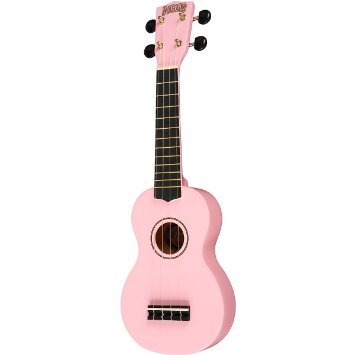
\includegraphics[width=5cm]{../img/ukulele.jpg}
\end{Slide}



\begin{Slide}{Koda i Scala}

  {\footnotesize\it Melodi: McDonalds-låten}

\begin{verbatim}

          G         C             G          D
Det finns stunder i livet som man alltid har kvar

          G           C               D
Det finns villkor och uttryck som man spar 

        A           D             A           E
Och där dörren står öppen finns gemenskap för fler 

A      D      E       A
Koda i Scala; det ger meeeeeeer! 
\end{verbatim}

\end{Slide}

\fi
